\section{Decision Trees}

Decision trees involve breaking down a dataset into smaller and smaller subsets. The result of this is a tree like structure containing decision nodes and leaf nodes.

\begin{figure}[H]
  \centering
  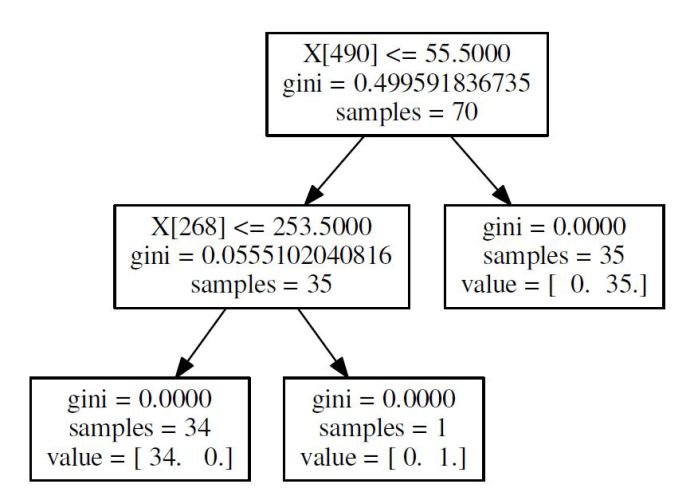
\includegraphics[scale=0.5,width=100mm]{./images/decision-tree-example.jpg}
  \caption{Example of a decision tree}
  \label{fig:abalone-decision-tree}
\end{figure}

Figure \ref{fig:abalone-decision-tree} taken from \cite{decisionTreeExample} shows a decision tree classification.The top level node is called the root, The middle row shows internal nodes and the bottom row shows 2 leaf nodes. Decision trees are basically a series of if/else clauses. The edges (black lines in figure \ref{fig:abalone-decision-tree}) represent either true or false.